% !TeX encoding = UTF-8

% \documentclass{article} % One-column default
\documentclass[twocolumn, switch]{article} % Method A for two-column formatting

\usepackage{preprint}

%% Math packages
\usepackage{amsmath, amsthm, amssymb, amsfonts}

%% Font
\usepackage{mathptmx}

%% Bibliography options

% \usepackage[numbers,square]{natbib}
% \bibliographystyle{apa}
%\usepackage{natbib}
\bibliographystyle{apacite}

%% General packages
\usepackage{verse}
\usepackage[LGR,T1]{fontenc}  % use 8-bit T1 fonts
\usepackage[utf8]{inputenc}	% allow utf-8 input
\newcommand{\textgreek}[1]{\begingroup\fontencoding{LGR}\selectfont#1\endgroup}
\usepackage{xcolor}		% colors for hyperlinks
\usepackage[colorlinks = false,
            linkcolor = purple,
            urlcolor  = blue,
            citecolor = cyan,
            anchorcolor = black]{hyperref}	% Color links to references, figures, etc.
\usepackage{booktabs,tabularx,graphicx} 		% professional-quality tables
\usepackage{nicefrac}		% compact symbols for 1/2, etc.
\usepackage{microtype}		% microtypography
\usepackage{lineno}		% Line numbers
\usepackage{float}			% Allows for figures within multicol
\usepackage{adjustbox}
\usepackage[hang,flushmargin]{footmisc} % no indents for footnotes

%\usepackage{multicol}		% Multiple columns (Method B)

\usepackage{apacite} % must be loaded after hyperref
\AtBeginDocument{\renewcommand{\APACrefYearMonthDay}[3]{\BBOP{#1}\BBCP}} % no months in citations ever
\usepackage{etoolbox}
\renewenvironment{APACrefURL}[1][]{}{}
\AtBeginEnvironment{APACrefURL}{\renewcommand{\url}[1]{}} % remove urls
\renewcommand{\doiprefix}{doi:~\kern-1pt} % want DOIs

\usepackage{lipsum}		%  Filler text

 %% Special figure caption options
\usepackage{newfloat}
\DeclareFloatingEnvironment[name={Supplementary Figure}]{suppfigure}
\usepackage{sidecap}
\sidecaptionvpos{figure}{l}
\usepackage{caption}
\captionsetup{justification=raggedright,singlelinecheck=false}

% Section title spacing  options
\usepackage{titlesec}
\titlespacing*{\section}{0pt}{0.5\baselineskip}{0.35\baselineskip}
\titlespacing*{\subsection}{0pt}{0.5\baselineskip}{0.25\baselineskip}
\titlespacing*{\subsubsection}{0pt}{0.5\baselineskip}{0.25\baselineskip}

\usepackage{changepage}

% ORCiD insertion
\usepackage{tikz,xcolor,hyperref}

\definecolor{lime}{HTML}{A6CE39}
\DeclareRobustCommand{\orcidicon}{
  
\begin{tikzpicture}
  \draw[lime, fill=lime] (0,0) 
  circle [radius=0.16] 
  node[white] {{\fontfamily{qag}\selectfont \tiny ID}};
  \draw[white, fill=white] (-0.0625,0.095) 
  circle [radius=0.007];
  \end{tikzpicture}
  \hspace{-2mm}
}
\foreach \x in {A, ..., Z}{\expandafter\xdef\csname orcid\x\endcsname{\noexpand\href{https://orcid.org/\csname orcidauthor\x\endcsname}
      {\noexpand\orcidicon}}
}
% Define the ORCID iD command for each author separately. Here done for two authors.
\newcommand{\orcidauthorA}{0000-0002-5214-7595}

% DSH submission requirements
% \usepackage{setspace} % spacing macros
% \doublespace
% \pagenumbering{gobble} % no page numbers for DSH
% \setlength{\parindent}{0.3in} % indent paras with no skip (gross)
% \setlength{\parskip}{0em}


%%%%%%%%%%%%%%%%   Title   %%%%%%%%%%%%%%%%
\title{Rhyme in Classical Latin Poetry: Stylistic or Stochastic?}

% Add watermark with submission status
\usepackage{xwatermark}
% Left watermark
% \newwatermark[firstpage,color=gray!60,angle=90,scale=0.32, xpos=-4.05in,ypos=0]{\href{https://doi.org/}{\color{gray}{Publication doi}}}
% Right watermark
% \newwatermark[firstpage,color=gray!60,angle=90,scale=0.32, xpos=3.9in,ypos=0]{\href{https://doi.org/}{\color{gray}{Preprint doi}}}
% Bottom watermark
\newwatermark[firstpage,color=gray!90,angle=0,scale=0.28, xpos=0in,ypos=-5in]{correspondence: \texttt{benjamin.nagy@adelaide.edu.au}}

%%%%%%%%%%%%%%%  Author list  %%%%%%%%%%%%%%%
\usepackage{authblk}
\renewcommand*{\Authfont}{\bfseries}
\author{Ben Nagy\orcidA{}}
\affil{
Department of Classics, Archaeology \& Ancient History

University of Adelaide
}

%%%%%%%%%%%%%%    Front matter    %%%%%%%%%%%%%%
\begin{document}

\twocolumn[ % Method A for two-column formatting
  \begin{@twocolumnfalse} % Method A for two-column formatting
  
\maketitle

\begin{abstract}
This study offers the first broad quantitative analysis of the use of rhyme in
classical Latin hexameter and elegiac verse. The data and tools developed for
the analysis are released under a permissive open source license. These
include: software to create an accurate phonetic transcription of Latin verse
from the MQDQ corpus; a system for scoring rhyme via phonetic similarity; and
a system for generating large amounts of metrically correct, stochastic Latin
verse (useful for analysis baselines). Further to this, some initial analysis
is performed: first via descriptive statistics and then with two unsupervised
multivariate analyses using dimension reduction methods. The study examines 19
works by 12 authors, comprising about 96 thousand lines. First and foremost,
the results show that rhyme was consciously used by classical authors, but to
different extents and in different ways. There is a solid and detectable
stylistic separation between the use of rhyme in elegy and epic, and possibly
also between satire and the rest. Within genres, authors can be stylistically
separated with a small set of features. On the negative side, it appears that
the stylistic signal from rhyme is fairly faint, and so forensic analysis
(e.g. for authorship attribution) is not presently recommended on texts that
are shorter than several thousand lines.\\

\textbf{Keywords}: Stylometry, Latin,
versification, rhyme, computational linguistics, corpus linguistics
\end{abstract}  %
\vspace{0.35cm}

  \end{@twocolumnfalse} % Method A for two-column formatting
] % Method A for two-column formatting

%\begin{multicols}{2} % Method B for two-column formatting (doesn't play well with line numbers), comment out if using method A


%%%%%%%%%%%%%%%  Main text   %%%%%%%%%%%%%%%
% \linenumbers

\section{Introduction}


There has long been a school of thought which holds that rhyme was not a
deliberate part of classical Latin poetics. The enormously influential
fouth-century commentator Servius remarked against \emph{Georgics} 3.539 that
he believed Vergil `mutavit genus, ut vitaret homoeoteleuton' (`changed the
gender [of \emph{timidi}] so that he could avoid homeoteleuton [`same ending'
in \emph{timidae}--\emph{dammae}]'). He makes similar claims against
\emph{Aen}. 5.391, 8.435, and 10.571. This belief that Latin poets avoided
rhyme, although not universally held, has persisted in various degrees to the
present day. The waters are muddied by the fact that `rhyme' is a slippery
term. One can certainly find discussion of it in the secondary literature, but
will also see euphemistic alternatives or related concepts: assonance,
consonance, euphony, homeoteleuton, or even the charmingly periphrastic
`vertical phonetic effects' \cite{vine_vertical_1989}. Further to this, what
does it mean for an author to `use' rhyme? It is certainly clear that
classical verse does not follow a formal scheme, and so which `sonic
correspondences' should be considered as rhyme and which as serendipity?
Finally, the classical corpus is substantial and there has not, previously,
been any way to identify rhymes short of carefully reading the text. This has
led to a fairly oblique debate in which proponents of rhyme cite one or two
striking examples while detractors assert coincidence.\footnote{
  For example, \citeA[32]{wilkinson_golden_1963} dismisses Propertius 2.34
  `where there are 38 examples of caesura-to-end rhyme\textellipsis in 94 lines,
  including six in succession' as `a freak'. A more fulsome consideration of the
  modern literature appears in Section \ref{sec:lit}.
}

This study intends to conclusively demonstrate that rhyme \emph{was} an aspect
of poetic style in classical Latin verse via several novel contributions. As a
necessary basis for automatic analysis, this paper presents the first public
implementation of correct (although simplified) phonetic transcription for
classical verse, including verse-specific features like elision
\cite{nagy_mqdq_2019}. Based on this, it suggests an initial algorithm for
scoring rhyme. Using these tools, some comparative analysis is performed on a
large corpus of classical hexameters and elegiac couplets (the two most common
metres)---19 works by 12 authors, comprising a total of 95,956 lines. No
previous work has performed a study of this breadth (a natural consequence of
the lack of automated analysis). The analysis provided is broad but
shallow---the main intent is to establish some fundamental facts and to
provide a basis for future work. Following an explanation of the key methods,
some descriptive statistics are examined and supplemented by an exploratory
multivariate analysis. First and foremost, the results show that rhyme
\emph{was} consciously used by classical authors, but to different extents and
in different ways. There is a solid and detectable stylistic separation
between the use of rhyme in elegy and epic, and possibly also between satire
and the rest. Within genres, authors can be stylistically separated with a
small set of features. All code and data is made freely available for extended
analysis work or for replication studies \cite{nagy_rhyme_2021}.

Of course there are some caveats. First and foremost it must be said that
statistical analysis is not in the business of determining `intention'. In
technical terms, this study does not answer the question of whether rhyme was
used `deliberately', only whether it was used `more often than chance could
produce'. Broadly speaking, the results of this study are statistically
conclusive, but fairly modest in scope. The methods described produce a
stylistic `fingerprint' that is fairly faint, and with significant variance.
Thus, while these results are encouraging, they are not yet sufficiently
robust for forensic purposes (e.g. authorship attribution).

\section{Relevant Literature}
\label{sec:lit}

\subsection{In `Traditional' Classics}

In this section I aim to direct the reader to \emph{some} of the most
important studies in `traditional' (by which in this case I mean non-digital)
Classics. An exhaustive treatment would be a significant work in itself, so I
aim rather to pick out the most quantifiable aspects of the literature, to use
as a basis for more rigorous analysis. To begin with the sceptics, the most
convincing treatment is \citeA{wilkinson_golden_1963} in \emph{Golden Latin
Artistry}. He includes a relatively lengthy consideration of the issues,
including a good representative selection of the arguments on both sides (such
as they existed at the time). In the final analysis, \citeA[32--3, inc.
nn]{wilkinson_golden_1963} is somewhat equivocal, but tends towards the view
that such rhymes as occur are not sought. Very valuably, however, he poses
exactly the right question (emphasis added):

\begin{adjustwidth}{0.1\linewidth}{0.1\linewidth}
  \footnotesize
  do [rhymes] occur \emph{in a greater
    degree than chance would produce}, given the nature of Latin terminations? To
  prove or disprove the proposition would require linguistic and statistical
  calculations of appalling complexity.
\end{adjustwidth}
In some senses, the entirety of the present study might be seen as a response
to this question; an attempt to perform the required calculations and finally
prove the proposition. One particular argument made by Wilkinson, on the
degree to which leonine\footnote{
  A rhyme between the word ending at the central caesura and the final word of
  the line---see Section \ref{sec:leo}. Unlike some other poetic traditions, a
  `caesura' occurs in Latin verse whenever a word ends inside a metrical foot.
  A `diaeresis' occurs when the end of a word and the end of a foot coincide.
}
rhymes are intentional is that, in some cases, Ovid appears to have
deliberately eschewed such rhymes---i.e. there are lines which could have
easily been arranged with this rhyme and yet were not.
\citeA[49]{platnauer_latin_1951} in one of the best-known treatments of
elegiac verse devotes just one page to `Pentameters with Internal Rhyme', in
which he makes much the same argument: `S.G. Owen in his note on Ov.
\emph{Tr.} \textsc{ii}. 104 implies that these rhymes were intentional, but a
cursory inspection of any of the poems shows that Ovid often failed to rhyme
where he could easily have done so; e.g. \textellipsis'. Both arguments share
the same fallacy. Simply because an author did not rhyme at every given
opportunity does not mean that they did not have a propensity to rhyme.

At the other end of the spectrum are the enthusiastic believers. Rosamund
\citeA{deutsch_1978} produced a well argued thesis on \emph{The Patterns of
Sound in Lucretius} in which she shows in careful detail a number of Lucretian
tendencies, including a chapter devoted to rhyme schemes (mostly vertical
schemes, although with some attention to the leonine style). There is much of
value in Deutsch's work, but it should be read in combination with its review
by Cyril \citeA{bailey_pattern_1939}. While I, too, am sceptical about the
hugely extended rhyme schemes Deutsch asserts (some rhyming associations are
claimed to occur more than fifty lines apart) the analysis presented in the
present study strongly supports her claim that Lucretius was a consistent and
deliberate user of vertical rhyme (also acknowledged by Bailey (p. 189):
`[t]hey are obvious in short passages'). For more in this vein, there is much
of interest in \citeA{guggenheimer_rhyme_1972}, in particular a strong review
of the historical background and a deft synthesis of the concepts across both
Latin and Greek verse. In some sections, again, Guggenheimer pushes the bounds
of credibility, but ideas must first be set out before they can be tested, so
it is an important work. Also indispensable is \citeA{herescu_poesie_1960},
although it still languishes without an English translation. Other authors
overstep the mark---\citeA[51]{clarke_intentional_1972} claims that `Vergil
and Ovid have \textellipsis placed internal and other rhymes [to emphasise
sense pauses] in the conclusions and beginning of clauses', but his methods
consider only the final syllable of the word (and so e.g. p. 58
\textbf{su}.cos is `rhymed' with \textbf{at}.ros and pe.\textbf{ti}.tos).
Given this, it is difficult to accept his main claim but none the less,
Clarke's section (pp. 55--72) on `concentrated' rhyme schemes is worthy of
attention. Also worth reading are \citeA{foster_certain_1909} on Propertius,
\citeA{skutsch_rhyme_1964} on Horace and \citeA{highet_sound-effects_1951} on
(mostly non-rhyme) sound effects in Juvenal.

\subsection{Computational Approaches}

Within computational stylometry itself, versification is an emerging area of
research and there is little existing work. It is covered in some detail in
\citeA{plechac_versification_2019} but the experiments described use a
probabilistic tagger which requires a seed corpus containing some rhyme in
predictable positions. While it is not directly relevant to this study,
readers may be interested in other fairly recent work that considers
versification; \citeA{marina_tarlinskaja_shakespeare_2016} on Shakespeare is
an important monograph, and provides a rare English language window into the
better established  `Russian school' of metrics;
\citeA{forstall_statistical_2019} have investigated some aspects of elegiac
metrical style; \citeA{nagy_hexml_2019} demonstrates the (very strong)
stylistic fingerprint in the metrical aspects of Latin hexameter. In terms of
computational approaches specific to rhyme in Latin verse, this study is, as
far as I am aware, the first. Since classical Latin verse did not follow a
formal scheme it seemed sensible to consider wider literature. In particular,
the study of `half-rhymes' and irregular schemes in rap music were extremely
useful. For English, the study by \citeA{hirjee_automatic_2009} uses a
probabilistic model based on a phonemic transcription. This improved their
accuracies for automatic detection of the highly interleaved and difficult
rhymes that are common to the genre. The following example is from p. 712
(rhymes are indicated by typeface):

\begin{adjustwidth}{0.1\linewidth}{0.1\linewidth}
  \footnotesize
\textbf{How I made it} you \textbf{salivated} over my \textbf{calibrated}\\
\textsc{raps} that \textbf{validated} my ghetto \emph{credibility}\\
\emph{Still I be} \textsc{pack}in \emph{agilities} \underline{unseen}\\
Forreal-a my killin \emph{abilities} \underline{unclean} \emph{facilities}\textellipsis\\
\begin{flushright}
Pharoahe Monch, \emph{Internal Affairs}
\end{flushright}
\end{adjustwidth}
Note how difficult some of these rhymes are to identify through orthography
alone, and the balance between `true' rhymes and half rhymes (\textsc{raps} /
\textsc{pack}in). Although this work was unknown to me at the time I wrote the
phonetic transcription and rhyme scoring (Section \ref{sec:findscore}), the
present study follows a similar approach in that it constructs a vowel and
consonant similarity matrix (cf. \citeA[713--4]{hirjee_automatic_2009}).
\citeA{kawahara_half_2007} follows a more formal linguistic approach, seeking
to detect `half-rhymes' in Japanese rap (again using a corpus containing known
rhymes). Kawahara's work is interesting in that it attempts to correlate
linguistic phonological features with an odds-ratio score for rhyme. Considering
shared features offers an empirical basis to consider phonemes to be `similar'.
As an example, in English /g/ and /k/ share the linguistic feature `velar'
(place of articulation) but differ in the feature `voice' (/g/ is voiced,
/k/ is not). \citeA[127]{kawahara_half_2007}, via multiple regression, shows
that some phonological features are more important than others when forming
rhymes. Some consideration of consonant features has been included, in
rudimentary fashion, in the scoring system used here, but further improvements
are almost certainly possible.

Considering the work on rap raises a possible improvement to the present
methods. In rhymes like `How I made it / salivated' (above) the correspondence
occurs in a continuous string of syllables, not on word boundaries---such an
approach might be interesting to pursue in future work on Latin. In
particular, it might provide an opportunity to engage with the ideas of
\citeA{ahl_metaformations_1985} on sub-word soundplay.

\section{Methodology}
\label{sec:methods}

\subsection{Producing a Phonetic Representation}

The first step in any analysis of rhyme is the conversion of the input text to
a phonetic representation. For modern languages, there are usually a variety
of available options, but this was not, unfortunately, the case for Latin. The
widely used, and generally extremely useful Classical Language Toolkit (CLTK)
(\citeA{johnsonetal2014}) offers, notionally, phonetic transcription, but its
performance was not strong enough for this analysis. The transcriber in the
CLTK (\texttt{cltk.phonology.latin.transcription}) suffers from three classes
of regular errors (over-formation of diphthongs, misplaced stress, and lack of
elision/prodelision) which make it unsuitable for the transcription of verse.
A key cause for some of these errors (and something outside the CLTK authors'
control) is that their analyser must cater heuristically for text where the
syllable count is unknown---in fact in Latin the correct syllabification is
sometimes impossible to determine without context (for example \emph{seruit}
might be [ser.wit] `he serves' or [se.ru.it] `she has joined').

For the present study, I was able to take advantage of the fact that the works
were drawn from the digital Musisque Deoque (MQDQ) corpus \cite{mqdq_2007},
which includes full scansion. Using this, I was able to perform accurate
syllabification. Then, by combining the MQDQ scansion with a modified version
of the CLTK code it was possible to produce a much better phonetic
representation. This code is included in the open-source Python package
\emph{MQDQParser} \cite{nagy_mqdq_2019} that accompanies the paper. The
precise phonetic representation (both in CLTK and in my own extensions) is
based on the reconstruction of \citeA{allen_vox_1965} but I chose a simplified
representation which omits many features that would be present in a `tight'
IPA transcription (rounding, dental `t's, consonant aspiration, etc.). These
did not seem to be relevant to rhyme. I retained nasalisation of final vowels,
but, for the sake of simplicity, \emph{not} vowel length, a choice which may
alarm some---so `peek' would rhyme with `pick'. \footnote{
  It would require a lengthy discursion to properly justify this decision, but,
  briefly: vowels in Latin poetry that we believe were pronounced short in
  normal speech are often scanned `long' (sometimes called `heavy') due to
  technical aspects of the metre. It is not clear how these were pronounced.
  Also, for a poet who wishes to create a sonic correspondence, vowel length can
  be stretched either way---these kinds of rhyme are easy to see in modern
  spoken-word poetry.
}
Vowels were mapped onto a Roman (aeiou) representation as opposed to an IPA
one; a transformation that has no effect on the analysis but is easier to
read.

\subsection{Finding and Scoring Rhyme}
\label{sec:findscore}

Although it may seem unbelievable, there does not appear to be any universally
agreed definition of `rhyme', or at least not in terms that are sufficiently
precise for practitioners who are tasked with measuring it. In general, one
could do much worse than to adopt the definitions from
\citeA{herescu_poesie_1960}. Herescu draws distinction between assonance and
rhyme (p. 136) in that assonance involves only the vowel; and between
homeoteleuton and rhyme in that homeoteleuton considers only the final
syllable whereas rhyme considers the final stressed syllable and every
syllable afterwards (p. 170--3). Having said that, I should make it clear that
I do not believe it is useful to draw such sharp distinctions when locating
and scoring `rhyme'.

My approach aimed at the generous discovery of sonic correspondences that
would be sensed as such by a regular speaker or listener, and not at any rigid
theoretical model. As will become clear, I would prefer to stretch the
appellation of a `rhyme' than to rule out on a technicality correspondences
which are obvious. So, to proceed: in this study two words were considered to
rhyme if they correspond in the syllabic nucleus (a vowel or diphthong, by
definition) of both their stressed and final syllables.\footnote{
  Note that in Latin, almost without exception, the final syllable in a
  multi-syllable word is unstressed, so the stressed and final syllables
  can only be identical in single syllable words. 
}
To `correspond', in this study is more permissive than `to match', and so /i/
and /e/ correspond quite closely (mid--high front vowels) as do /ae/ and /e/
(identical place of articulation at the end of the diphthong). For words with
two syllables following the stress, a pedantically perfect rhyme would require
correspondence in both---this I have not enforced, and so
`\textbf{pro}.ba.ble' and `\textbf{hor}.ri.ble' would achieve an almost
perfect score. Additionally I have permitted, with a penalty, words with
mismatched `tails'. This allows `slurred' rhymes of the form
`\textbf{ca}.li.dus' and `\textbf{cal}.dus'. From a phonetic point of view,
this is natural in speech. For classical Latin in particular, it is supported
by Quintillian, who reports that `Augustus again in his letters to Gaius
Caesar corrects him for preferring calidus to caldus, not on the ground that
the former is not Latin, but because it is unpleasing and as he himself puts
it in Greek \textgreek{περίεργον} (affected)' (Quint. \emph{Inst.} 1.6.19,
transl. Butler). In short, I accept under the broad moniker of `rhyme' a
fairly rag-tag bunch of homophonies that would be called a variety of
different things by other authors.

In fact, the system goes even further. Instead of a binary classification
(rhyming or not), rhymes were scored. The score is based mostly on the
`closeness' of the vowels, but also considers the onset of the final syllable
and the coda of both the final and the stressed syllable. Similar approaches
can be seen in the work which focused on rap, where imperfect rhymes are
extremely common (as discussed above). A vowel similarity matrix was
constructed from first principles,\footnote{
  Unlike the related work by \citeA{hirjee_automatic_2009} and
  \citeA{kawahara_half_2007} there is no corpus of classical Latin verse
  containing known rhymes to use as a training set for a deep-learning or
  probabalistic approach.
}
using the phonetic vowel positions (i.e. the positions on a two-dimensional
formant frequency plot, as can be seen in any introduction to phonology). The
similarity for consonants was decided using broad linguistic features
(alveolar, velar, voiced, unvoiced etc.). Finally, some bonuses were applied
for perfect matches, and the final syllable was weighted slightly more than
the stressed syllable (based on subjective feedback). Of course there is a
great deal of imprecision, here, and so the scoring system went through a
number of tuning phases in which experienced Latinists were asked to review
the rhyme scores. This approach may not seem particularly scientific and
objective, but (I argue) neither is the human experience of rhyme. Even poets
might be expected to disagree on the quality of this rhyme or that and so a
computer can hardly be expected to produce a perfect result. What is most
important is that the scores can be applied systematically and consistently.
For reference, Table \ref{tab:scores} presents the automatic analysis and
rhyme scores for twenty-five random pairs of words that exceed the global
threshold for a `rhyme' as defined in this study. The rhymes with scores near
the lower threshold are, by definition, `barely rhymes'.

\begin{table}[h!]
\caption{
Phonetic analysis and calculated rhyme scores for twenty-five random word
pairs. The final score is composed of one score for the stressed
syllable and another for the final syllable. Higher scores are better, maximum
possible is 2.30, minimum threshold is 1.75.
}
\label{tab:scores}
\par\smallskip
\resizebox{\linewidth}{!}{
\begin{tabular}{llllc@{\hspace{2\tabcolsep}}c@{\hspace{0.75\tabcolsep}}c}
\toprule
     \multicolumn{2}{c}{Orthographic} & \multicolumn{2}{c}{Phonetic} & Score &  (Stress  /&Final) \\
\midrule
       pingues &    puerique &           \textbf{ping}.wes &   pu.e.\textbf{rī}.kwe &   1.77 &    0.72 &   1.05 \\
     sortemque &     tristes &        sor.\textbf{tem}.kwe &       \textbf{tris}.tes &   1.77 &    0.60 &   1.17 \\
     erroribus &    callidus &     ēr.\textbf{rō}.ri.bus &     \textbf{kal}.li.dus &   1.78 &    0.48 &   1.30 \\
           ait &       redit &               \textbf{a}.it &         \textbf{red}.it &   1.78 &    0.48 &   1.30 \\
          apte &  pariterque &             \textbf{āp}.te &  pa.ri.\textbf{ter}.kwe &   1.78 &    0.48 &   1.30 \\
         habet &     sparsit &             \textbf{ha}.bet &       \textbf{spar}.sit &   1.79 &    0.80 &   0.99 \\
       inpetus &   frondibus &         \textbf{īn}.pe.tus &    \textbf{fron}.di.bus &   1.80 &    0.50 &   1.30 \\
    herbosaque &       foret &     her.\textbf{bō}.sa.kwe &         \textbf{fo}.ret &   1.87 &    1.00 &   0.87 \\
         fetus &      iratus &            \textbf{fē}.tus &     ī.\textbf{rā}.tus &   1.90 &    0.60 &   1.30 \\
 anguiferumque &        uoce &  ang.wi.fe.\textbf{rum}.kwe &         \textbf{wō}.ke &   1.90 &    0.60 &   1.30 \\
        recens &      ingens &            \textbf{re}.kens &       \textbf{īn}.gens &   1.90 &    0.60 &   1.30 \\
         caede &     uetuere &             \textbf{kae}.de &    we.tu.\textbf{ē}.re &   1.92 &    0.70 &   1.22 \\
       habebat &      iniqua &         ha.\textbf{bē}.bat &      i.\textbf{nī}.kwa &   1.92 &    0.75 &   1.17 \\
     nouissima &       media &       no.\textbf{wis}.si.ma &       \textbf{me}.di.ā &   1.93 &    0.71 &   1.22 \\
    certaminis &       satis &     ker.\textbf{tā}.mi.nis &         \textbf{sa}.tis &   1.95 &    1.00 &   0.95 \\
          mihi &      digiti &             \textbf{mi}.hī &      \textbf{di}.gi.tī &   1.95 &    1.00 &   0.95 \\
         dixit &     accessi &            \textbf{dik}.sit &    āk.\textbf{kes}.sī &   2.01 &    0.71 &   1.30 \\
      manumque &       forte &         ma.\textbf{num}.kwe &         \textbf{for}.te &   2.01 &    0.71 &   1.30 \\
         verba &     bellica &             \textbf{wer}.ba &      \textbf{bel}.li.ka &   2.03 &    0.95 &   1.08 \\
         serta &     solebat &             \textbf{ser}.ta &     so.\textbf{lē}.bat &   2.04 &    0.80 &   1.23 \\
      praebuit &    aequoris &         \textbf{prae}.bu.it &     \textbf{ae}.kwo.ris &   2.05 &    1.00 &   1.05 \\
         damni &       magni &             \textbf{dam}.ni &         \textbf{man}.ji &   2.17 &    0.95 &   1.22 \\
         curis &       putes &            \textbf{kū}.ris &         \textbf{pu}.tes &   2.17 &    1.00 &   1.17 \\
         rogum &    cyclopum &            \textbf{ro}.g\~{u}m &    kü.\textbf{klo}.p\~{u}m &   2.30 &    1.00 &   1.30 \\
       sororum &       locum &        so.\textbf{rō}.r\~{u}m &        \textbf{lo}.k\~{u}m &   2.30 &    1.00 &   1.30 \\
\bottomrule
\end{tabular}
}
\end{table}

\subsection{Which Rhymes to Look For?}
\label{sec:which_rhymes}

The next determination was to select a set of target rhymes. The leonine
pattern was clearly interesting, because it is considered in most of the
traditional literature. End rhymes were another obvious target, since they
form the basis for structured rhyme in many languages. I also chose to
investigate initial rhymes, because of the convincing arguments put by
\citeA[121 ff.]{deutsch_1978} concerning the use of this feature by Lucretius.
After that, some investigation was required. There is no reason to suppose
that Latin poets should follow modern traditions, if indeed they consciously
engaged in rhyme at all. With this in mind, I investigated the work of
multiple poets with a variety of rhyme-search functions. These search
functions are named as follows: for rhymes that occur in two different lines,
the matching lines are denoted `a' and the intervening lines `x'. The position
(for vertical rhymes) is denoted with an index, `0' for the first word, `-1'
for the final word, `-2' for the penultimate, `mid' for the word ending at the
central caesura. Thus the search \texttt{axxa -2} would look for a rhyme in
the penultimate word at the first and last lines of a quatrain. Patterns that
were investigated but which do not appear in the study include `chiastic'
rhymes where, for example, the midword rhymes with the end of the following
line, and ante-penultimate rhymes (`-3'). Those rhymes do occur (as chance
insists they must) but did not appear to be present to an interesting degree.
However, ante-penultimate rhymes do occur from time to time in the rarer mosaic
rhymes (Section \ref{sec:mosaic}), and so further studies of mosaic rhymes in
particular might be wise to consider them. The final set of searches that were
performed for each work can be seen in Table \ref{tab:df_apot} (an example
analysis for Prudentius' \emph{Apotheosis}) in the `Test' column.

\subsection{The Propensity Index (\texorpdfstring{$\Pi$}{PI})}

Having determined which rhymes to consider, the next problem is how to
determine whether these rhymes occur more (or less) than chance would suggest.
A simplistic approach (the obvious one being a simple percentage) would be
deceptive here for a number of reasons. The most important observation is that
the lexical set (and hence the expected number of rhymes) differs not only by
author, but also by word position. In Latin verse, the ends of the lines
generally fall into correspondence between the word stress (the ictus) and the
foot patterns (the accent). To put it inelegantly, the stress pattern for the
end of a line is typically `DUM di di DUM dum'. Fitting words to this stress
pattern (which also possess the required syllable quantities) constrains the
available lexicon for both the penultimate and the final position. The effect
of this constraint is that the baseline expectation for rhyme is much higher
for penultimate words and finals. In the \emph{Metamorphoses}, for example, if
one selects two final words at random they will rhyme around 7.4\% of the
time; for penultimate words the figure is about 9.6\%, whereas for the
relatively unconstrained set of initial words the figure is just 3.9\%.
Clearly, then, we cannot simply compare percentages, because some positions,
as well as some authors, are `rhymier' than others.

To address this, the figures in this study are based on the \emph{propensity}
of an author to rhyme in a given position, considering the number of observed
rhymes as compared to the number expected. This measure was dubbed the
Propensity Index and is denoted `$\Pi$' throughout. If there are twice as many
rhymes of a certain type as chance would suggest then the $\Pi$ score would be
2.0. A score of less than 1.0 indicates a negative preference. For many
readers, the question that immediately arises will be `how are the expected
values determined?'---and this will be discussed in the following sections.
Broadly speaking, $\Pi$ is similar to the `odds ratio', but not precisely
the same; it was therefore thought less confusing to introduce the burden of
new terminology than to provide a lengthy explanation of the ways in which I
have deviated from a textbook measure. The essential motivation for the
changes is that the odds ratio can exhibit significant variance when dealing
with rare events, especially with fairly small sample sizes. For this study a
more robust measure of expectation was therefore seen to be critical.

\subsection{Building the Binomial (Theoretical) Model} 

Now we come to the nub of the motivating question. As put by \citeA[33 (in
note)]{wilkinson_golden_1963}: `do [rhymes] occur in a greater degree than
chance would produce'? So, just how many rhymes \emph{would} chance produce?
This study constructs two models so that the results can be compared and
cross-validated. This section describes the theoretical model based on a
binomial distribution, the next describes an empirical (simulated) model. For
the binomial model, we first estimate the probability with which any two words
(from just the set of words appearing in that position) rhyme. For a set of
\emph{n} words, this yields $n(n-1)$ pairs, a potentially large number. In
cases where the sets were prohibitively large, the probability was taken to be
the median of the probabilities calculated from 100 sets of 50,000 random
pairs. This supplies us with a notional `ground truth'.

Next, to derive an expected number of rhymes, the problem is modelled as a
series of Bernoulli trials, in which each eligible pair of words should rhyme
(or not) with some baseline probability \emph{P}. The expected number of
rhymes can then be calculated using the binomial distribution, or
alternatively, the $P$-value for any given observation can be calculated the
same way (using a standard binomial test).\footnote{
  In the included tables, the binomial $P$-values have been calculated using a
  `one-sided' binomial test. The `two-sided' test tells us whether it is likely
  that an observed score is within a sensible range (higher or lower). For the
  present purposes it was more interesting to know specifically whether an
  observation was unusually high \emph{or} low.
}
There are some theoretical concerns with this construction. In the first
place, the eligible pairs overlap. In looking for couplet rhymes (\texttt{aa
-1}) we would consider the pairs of lines numbered \{(1,2), (2,3), (3,4)
\textellipsis\}---this means that the trials are not independent. Further,
there are many other factors which might make it more or less likely for a
position to rhyme as compared to the baseline. A line of Latin verse is a
complicated compromise between quantity, rhythm, caesurae, diaereses and any
number of other factors which impose conditions as to which words may be
placed in which positions. In view of these potential issues with the binomial
model, it was sensible to cross-check the results.

\subsection{Building the (Simulated) Null Model} 

To better understand the plausibility of the theoretical model I then set out
to construct a simulated model that would build stochastic Latin verse. The
aim was to produce verse that obeyed the formal rules (and also respected the
informal ones like foot distribution, caesura positions, and ictus/accent
conflict) but paid no attention to semantic or grammatical content. As a
curiosity, I note that there is some precedent to this effort, although not
for the same reasons (nor with the same properties). The `Eureka Machine' in
1845 used a series of mechanical drums inscribed with various Latin words to
create lines of random hexameter, to the amusement of many (and for the
admission price of one shilling).\footnote{
  For a detailed and entertaining account of the Eureka, see 
  \citeA{blandford_eureka_1963}
}
Eureka created verses according to a fixed grammatical (and metrical) pattern
(\textsc{adj}, \textsc{n}, \textsc{adv}, \textsc{v}, \textsc{n},
\textsc{adj}), and so such an approach would hardly possess the properties
needed here. Instead, I once again made use of the fact that the MQDQ corpus
is fully scanned, and so for every word there is metadata recording its
metrical position in the line (e.g. a word might start at the beginning of a
second-foot spondee and end at the first breve of a third-foot dactyl). This
allowed words to be `stitched together'. After selecting a random first word,
the code selects another word which begins at the correct metrical position,
and thus continues until an entire line has been created. Of course it is not
quite so simple---not all words can be joined, because they must also respect
the rules for elision (a word that does not begin with a vowel cannot be
joined to a word that ends with elision) and quantity (a word ending with a
short syllable and a consonant final cannot be followed by a word that begins
with a consonant, otherwise the syllable would have `lengthened by position').
The final output has the very desirable quality that it respects metrical
style to a fairly high degree. For example, since Ovid almost never writes a
line without a third-foot caesura, there is almost no chance that the
simulator will construct one. An example of the output can be seen in Fig.
\ref{fig:ps_tib}.\footnote{
  The translation, although still somewhat vexed, assumes the following
  grammatical emendments: for \emph{Coa}, Coas; for \emph{mihi}, mei (gen. of
  cause); for \emph{sobrius}, sobria; for \emph{exsequias}, exsequia.
}

\begin{figure}[h!]
\caption{
Two elegiac couplets from Simulated Tibullus. The content is nonsense, but an
attempted `translation' is supplied. Emphasised words indicate that the
grammatical form does not quite match the translation.
}
\label{fig:ps_tib}
\par\medskip
\footnotesize
\centering
\begin{tabular}{l}
at frustra custodit anus: mihi, \emph{Coa} poetas!\\
\phantom{xx} praemoneo, uinclis iam super illa cubet.\\
at \emph{mihi} paeniteat sortes, mea \emph{sobrius} aetas,\\
\phantom{xx} nempe age! praedico, flebitur \emph{exsequias}.
\\
\phantom{xxx}\\
The old woman guards in vain: the poets of Cos are mine!\\
\phantom{xx} I warn you, let her sleep now above the chains.\\
Yet if chance is against me, my sober age,\\
\phantom{xx} well then do it! I foresee weeping at my funeral.\\
\end{tabular}
\end{figure}

Given this software, it was now possible to create a `null model' which
produced lines by chance, and yet was still constrained by the technical and
conventional features of the medium. From there it was a simple (although
computationally intensive) matter to simulate a `pseudo \emph{Aeneid}' or a
`pseudo \emph{Pharsalia}' and count the number of each kind of rhyme that
occurred. The chosen approach was to produce 101 simulated texts, each
matching the length of its original, and then use the median count as the
statistic for the expected number of rhymes. There is more variation in the
expected values from shorter texts (as can be seen in the distances between
the high and low 95\textsuperscript{th} percentiles (H$_{95}$ and L$_{95}$)).
This was a deliberate choice (more text could easily have been simulated)
because the results for the smaller texts probably \emph{are} less reliable,
and so there is no sense in obscuring the fact. Observed results were then
marked with a significance level using stars (which are much loved by users of
statistical software). For a result outside the 90\textsuperscript{th}
(simulated) percentile, one star, and another for the 95\textsuperscript{th}
and the 99\textsuperscript{th}.

Comfortingly, the simulated and theoretical models correspond fairly closely.
In particular, differences of opinion regarding the levels of significance
(0.1, 0.05, 0.01) are quite rare. For the $\Pi$ scores, I chose to use
expected values from the simulated model because it tends to be more
conservative than the binomial, but probably either approach would have been
reasonable. The binomial model is certainly quicker to calculate, but it is
much less flexible. Some baseline probabilities are essentially impossible to
calculate (see the discussion of the \texttt{slant\_leo} test in section
\ref{sec:leo}), whereas the results of any rhyme search are as easy to count
in the simulated lines as in the original text.

\subsection{The Rhyminess of Whole Texts}
\label{sec:whole_rhyminess}

In section \ref{sec:which_rhymes}, we explored the individual rhyme tests that
were applied to each work. Works were also characterised by two more
statistics---global measures (mean per-line) for \texttt{rhyme amount} and
\texttt{rhyme strength}. The former is intended to express rhyme
\emph{density} and the latter to capture the degree to which an author would
use clearly obvious rhymes (disparagingly called `jingles'). In the
meta-analysis of the multi-variate models these scores are strongly
correlated, and so perhaps this could have been captured in a single
statistic, but some authors have a bias towards one or the other feature,
so for now they remain distinct.

The scoring algorithm is fairly straightforward. The scanner proceeds
word-by-word and marks all words within a four line window which qualify as a
vertical or leonine rhyme. The best rhyme for each word is then used for the
final mean. For the purposes of manual investigation, rhymes are also assigned
a deterministic colour, calculated based on the nuclei of the syllables which
constitute the rhyme (as can be seen in Figs \ref{fig:mosaic_phars},
\ref{fig:mosaic_aen} and \ref{fig:phars_barely}). The scoring calculation is
configurable, allowing the software to scan for the `best' leonine rhymes,
mid-rhymes, general mosaics etc. Finally, and unlike the $\Pi$ scores, these
rhyme scores are \emph{z}-transformed and standardised to a zero mean and unit
variance before being included in the cluster analysis (without this step they
completely dominate the cluster output).

\begin{table*}[h!]
\caption{An example analysis for a single work (Prudentius' \emph{Apotheosis})}
\label{tab:df_apot}
\par\medskip
\centering
\resizebox{0.9\linewidth}{!}{
  \begin{tabular}{lclcccclcc@{\hspace{1\tabcolsep}}c@{\hspace{1\tabcolsep}}c}
  \toprule
        &&&&&&\multicolumn{3}{c}{Theoretical (Binomial)}&\multicolumn{3}{c}{Simulated}\\\cmidrule(lr{2pt}){7-9}\cmidrule(l{2pt}r){10-12}
      Work & Metre &       Test &    $\Pi$ & Signif. &    Obs. &  Exp. & Alt. &  $P$-val & L$_{95}$ &  M$_{50}$ &  H$_{95}$ \\
  \midrule
 Apotheosis &     H &  \texttt{      leo} & 1.6667 &   *** &   90 &        53 &     greater & <0.0001 &       39 &   54 &   68 \\
 Apotheosis &     H &  \texttt{  slant leo} & 1.2368 &       &   47 &         - &        -    & -      &       27 &   38 &   50 \\
 Apotheosis &     H &  \texttt{     aa 0} & 1.5294 &   *** &   52 &        35 &     greater & 0.0038 &       23 &   34 &   46 \\
 Apotheosis &     H &  \texttt{    axa 0} & 1.1667 &       &   42 &        35 &     greater & 0.1341 &       24 &   36 &   48 \\
 Apotheosis &     H &  \texttt{   axxa 0} & 1.1622 &       &   43 &        35 &     greater & 0.1012 &       26 &   37 &   49 \\
 Apotheosis &     H &  \texttt{    aa -1} & 1.0597 &       &   71 &        69 &     greater & 0.4161 &       51 &   67 &   84 \\
 Apotheosis &     H &  \texttt{   axa -1} & 1.0882 &       &   74 &        69 &     greater & 0.2782 &       56 &   68 &   86 \\
 Apotheosis &     H &  \texttt{  axxa -1} & 1.0441 &       &   71 &        69 &     greater & 0.4099 &       54 &   68 &   83 \\
 Apotheosis &     H &  \texttt{    aa -2} & 1.1778 &       &  106 &        90 &     greater & 0.0433 &       73 &   90 &  110 \\
 Apotheosis &     H &  \texttt{   axa -2} & 1.1957 &     * &  110 &        90 &     greater & 0.0161 &       73 &   92 &  111 \\
 Apotheosis &     H &  \texttt{  axxa -2} & 0.9785 &       &   91 &        90 &     greater & 0.4514 &       76 &   93 &  110 \\
 Apotheosis &     H &  \texttt{   aa mid} & 1.1754 &       &   67 &        55 &     greater & 0.0551 &       43 &   57 &   74 \\
 Apotheosis &     H &  \texttt{  axa mid} & 1.0741 &       &   58 &        55 &     greater & 0.3431 &       41 &   54 &   68 \\
 Apotheosis &     H &  \texttt{ axxa mid} & 1.2143 &     * &   68 &        55 &     greater & 0.0408 &       43 &   56 &   70 \\
  \bottomrule
  \end{tabular}
}
\end{table*}

\section{Results}
\label{sec:results}

\subsection{Some Initial Univariate Analysis}

\begin{table*}[h!]
\caption{
  Which vertical rhymes did classical Latin poets prefer? A table of works which
  show a statistically significant propensity ($\Pi$) for the given rhymes.
  Leonine features are not included because almost all works exhibit them, see
  Table \ref{tab:leo} for that analysis. This includes complete works only,
  where the statistics are less variable.
}
\label{tab:allbutleo}
\par\medskip
\centering
\begin{adjustbox}{totalheight=0.9\textheight}
  \begin{tabular}{lclcccclcc@{\hspace{1\tabcolsep}}c@{\hspace{1\tabcolsep}}c}
  \toprule
          &&&&&&\multicolumn{3}{c}{Theoretical (Binomial)}&\multicolumn{3}{c}{Simulated}\\\cmidrule(lr{2pt}){7-9}\cmidrule(l{2pt}r){10-12}
          Work & Metre &       Test &    $\Pi$ & Signif. &    Obs. &  Exp. & Alt. &  $P$-val & L$_{95}$ &  M$_{50}$ &  H$_{95}$ \\
  \midrule
        Aeneid &     H &   axxa -1 & 1.0789 &      ** &   779 &   723 &  greater &  0.0161 &      674 &      722 &      767 \\
        Aeneid &     H &    axxa 0 & 1.1040 &       * &   276 &   251 &  greater &  0.0589 &      229 &      250 &      279 \\
    Apotheosis &     H &      aa 0 & 1.5294 &     *** &    52 &    35 &  greater &  0.0038 &       23 &       34 &       46 \\
    Apotheosis &     H &    axa -2 & 1.1957 &       * &   110 &    90 &  greater &  0.0161 &       73 &       92 &      111 \\
    Apotheosis &     H &  axxa mid & 1.2143 &       * &    68 &    55 &  greater &  0.0408 &       43 &       56 &       70 \\
   Argonautica &     H &  axxa mid & 0.8967 &      ** &   269 &   304 &     less &  0.0183 &      271 &      300 &      331 \\
           Ars &     H &      aa 0 & 2.3889 &     *** &    86 &    37 &  greater &  <0.0001 &       25 &       36 &       49 \\
           Ars &     H &     axa 0 & 1.4872 &      ** &    58 &    38 &  greater &  0.0012 &       27 &       39 &       49 \\
           DRN &     H &     aa -1 & 1.2597 &     *** &   679 &   563 &  greater &  <0.0001 &      504 &      539 &      584 \\
           DRN &     H &     aa -2 & 1.0908 &      ** &   697 &   652 &  greater &  0.0356 &      585 &      639 &      694 \\
           DRN &     H &      aa 0 & 1.1770 &     *** &   246 &   205 &  greater &  0.0028 &      175 &      209 &      235 \\
           DRN &     H &    aa mid & 1.1279 &     *** &   291 &   256 &  greater &  0.0160 &      227 &      258 &      288 \\
           DRN &     H &    axa -1 & 1.1648 &     *** &   636 &   563 &  greater &  0.0009 &      498 &      546 &      589 \\
           DRN &     H &     axa 0 & 1.1699 &       * &   241 &   205 &  greater &  0.0075 &      185 &      206 &      241 \\
           DRN &     H &   axxa -1 & 1.1447 &     *** &   625 &   563 &  greater &  0.0040 &      496 &      546 &      592 \\
           DRN &     H &   axxa -2 & 1.0853 &     *** &   687 &   652 &  greater &  0.0795 &      583 &      633 &      683 \\
           DRN &     H &  axxa mid & 1.1313 &       * &   293 &   256 &  greater &  0.0116 &      227 &      259 &      298 \\
         Fasti &     H &     aa -2 & 1.1220 &     *** &   285 &   251 &  greater &  0.0146 &      231 &      254 &      283 \\
         Fasti &     H &      aa 0 & 1.4125 &     *** &   113 &    83 &  greater &  0.0010 &       65 &       80 &      100 \\
         Fasti &     P &      aa 0 & 1.2262 &       * &   103 &    83 &  greater &  0.0191 &       65 &       84 &      106 \\
         Fasti &     H &     axa 0 & 1.3913 &     *** &   128 &    91 &  greater &  0.0001 &       71 &       92 &      114 \\
         Fasti &     H &    axxa 0 & 1.2976 &      ** &   109 &    83 &  greater &  0.0035 &       69 &       84 &      100 \\
      Georgics &     H &    axa -2 & 1.1408 &      ** &   235 &   205 &  greater &  0.0173 &      179 &      206 &      232 \\
  Hamartigenia &     H &     axa 0 & 1.3333 &       * &    36 &    26 &  greater &  0.0339 &       17 &       27 &       37 \\
  Hamartigenia &     H &    axxa 0 & 1.3462 &       * &    35 &    26 &  greater &  0.0493 &       16 &       26 &       36 \\
      Heroides &     H &      aa 0 & 2.0000 &     *** &   116 &    59 &  greater &  <0.0001 &       46 &       58 &       81 \\
      Heroides &     P &      aa 0 & 1.4000 &     *** &    84 &    59 &  greater &  0.0012 &       45 &       60 &       75 \\
      Heroides &     H &    aa mid & 1.1887 &       * &   126 &   105 &  greater &  0.0221 &       85 &      106 &      126 \\
      Heroides &     P &    aa mid & 1.2336 &     *** &   132 &   105 &  greater &  0.0052 &       86 &      107 &      122 \\
      Heroides &     H &     axa 0 & 1.6230 &     *** &    99 &    59 &  greater &  <0.0001 &       47 &       61 &       75 \\
     Hor. Sat. &     H &    axa -1 & 1.2049 &      ** &   147 &   131 &  greater &  0.0770 &       91 &      122 &      143 \\
     Hor. Sat. &     H &   axxa -1 & 1.2720 &     *** &   159 &   131 &  greater &  0.0069 &      105 &      125 &      144 \\
 Metamorphoses &     H &     aa -1 & 1.0544 &       * &   949 &   884 &  greater &  0.0127 &      854 &      900 &      962 \\
 Metamorphoses &     H &     aa -2 & 1.0629 &      ** &  1234 &  1145 &  greater &  0.0033 &     1091 &     1161 &     1233 \\
 Metamorphoses &     H &      aa 0 & 1.1970 &     *** &   553 &   462 &  greater &  <0.0001 &      421 &      462 &      507 \\
 Metamorphoses &     H &    aa mid & 1.1252 &     *** &   692 &   603 &  greater &  0.0001 &      555 &      615 &      674 \\
 Metamorphoses &     H &    axa -1 & 1.0656 &      ** &   959 &   884 &  greater &  0.0049 &      843 &      900 &      950 \\
 Metamorphoses &     H &    axa -2 & 1.0434 &       * &  1203 &  1145 &  greater &  0.0381 &     1098 &     1153 &     1206 \\
 Metamorphoses &     H &     axa 0 & 1.0919 &      ** &   511 &   462 &  greater &  0.0109 &      436 &      468 &      510 \\
     Pharsalia &     H &      aa 0 & 1.1028 &       * &   279 &   254 &  greater &  0.0645 &      221 &      253 &      283 \\
     Pharsalia &     H &    axa -2 & 1.0907 &     *** &   926 &   846 &  greater &  0.0023 &      801 &      849 &      897 \\
     Pharsalia &     H &    axxa 0 & 1.1641 &     *** &   298 &   254 &  greater &  0.0036 &      225 &      256 &      287 \\
    Propertius &     P &     aa -1 & 0.8794 &       * &   124 &   138 &     less &  0.1228 &      121 &      141 &      159 \\
    Propertius &     H &     aa -2 & 1.1391 &      ** &   262 &   228 &  greater &  0.0093 &      200 &      230 &      257 \\
    Propertius &     H &      aa 0 & 1.9592 &     *** &    96 &    51 &  greater &  <0.0001 &       35 &       49 &       65 \\
    Propertius &     P &      aa 0 & 1.3125 &       * &    63 &    51 &  greater &  0.0525 &       39 &       48 &       63 \\
    Propertius &     P &    aa mid & 0.8226 &      ** &   102 &   122 &     less &  0.0346 &      105 &      124 &      146 \\
    Propertius &     H &    axa -2 & 1.2732 &     *** &   247 &   195 &  greater &  0.0001 &      170 &      194 &      224 \\
    Propertius &     P &    axa -2 & 1.1168 &      ** &   392 &   344 &  greater &  0.0027 &      317 &      351 &      389 \\
    Propertius &     H &     axa 0 & 1.7885 &     *** &    93 &    53 &  greater &  <0.0001 &       42 &       52 &       68 \\
    Propertius &     P &   axxa -2 & 1.1013 &       * &   250 &   228 &  greater &  0.0623 &      205 &      227 &      258 \\
    Propertius &     P &    axxa 0 & 1.3400 &      ** &    67 &    51 &  greater &  0.0158 &       36 &       50 &       66 \\
  Psychomachia &     H &      aa 0 & 0.7308 &       * &    19 &    26 &     less &  0.0937 &       17 &       26 &       38 \\
  Psychomachia &     H &     axa 0 & 1.5385 &     *** &    40 &    26 &  greater &  0.0056 &       18 &       26 &       38 \\
  Psychomachia &     H &   axxa -1 & 1.2388 &      ** &    83 &    66 &  greater &  0.0171 &       52 &       67 &       81 \\
        Punica &     H &     aa -1 & 0.9287 &      ** &   860 &   924 &     less &  0.0138 &      867 &      926 &      981 \\
        Punica &     H &   axxa -2 & 1.0448 &       * &  1260 &  1206 &  greater &  0.0528 &     1135 &     1206 &     1267 \\
        Punica &     H &  axxa mid & 1.0807 &      ** &   576 &   536 &  greater &  0.0421 &      473 &      533 &      571 \\
       Thebaid &     H &    axa -1 & 1.0578 &       * &   787 &   739 &  greater &  0.0348 &      692 &      744 &      798 \\
       Thebaid &     H &    axa -2 & 1.0577 &       * &  1009 &   954 &  greater &  0.0315 &      886 &      954 &     1019 \\
      Tibullus &     H &      aa 0 & 2.3750 &     *** &    38 &    17 &  greater &  <0.0001 &       10 &       16 &       24 \\
      Tibullus &     P &      aa 0 & 1.5625 &      ** &    25 &    17 &  greater &  0.0301 &        9 &       16 &       24 \\
      Tibullus &     H &     axa 0 & 2.2727 &     *** &    50 &    21 &  greater &  <0.0001 &       15 &       22 &       30 \\
      Tibullus &     P &   axa mid & 1.2353 &       * &    63 &    49 &  greater &  0.0240 &       34 &       51 &       64 \\
      Tibullus &     P &   axxa -1 & 0.8372 &       * &    36 &    44 &     less &  0.1296 &       34 &       43 &       55 \\
       Tristia &     H &      aa 0 & 1.4737 &     *** &    84 &    58 &  greater &  0.0006 &       45 &       57 &       72 \\
       Tristia &     H &     axa 0 & 1.5902 &     *** &    97 &    61 &  greater &  <0.0001 &       48 &       61 &       75 \\
       Tristia &     P &     axa 0 & 1.2687 &     *** &    85 &    64 &  greater &  0.0068 &       51 &       67 &       79 \\
       Tristia &     H &   axa mid & 1.1647 &       * &    99 &    84 &  greater &  0.0546 &       67 &       85 &      102 \\
       Tristia &     H &   axxa -2 & 1.1414 &       * &   218 &   188 &  greater &  0.0139 &      171 &      191 &      219 \\
  \bottomrule
  \end{tabular}
\end{adjustbox}
\end{table*}

\subsubsection{Vertical Rhymes (Table \ref{tab:allbutleo})} 

Vertical end-rhymes were not heavily sought, but neither were they avoided.
The most enthusiastic user of them is Lucretius in \emph{De Rerum Natura}.
Horace also has a propensity for this type, and it occurs in Vergil
and Ovid, although at the very edge of what might be called a plausible
coincidence. None of the later epicists appear to favour end-rhymes although
it is very interesting to note that Silius Italicus is the only hexameter
author to show a negative propensity for the `couplet' style (feature
\texttt{aa -1}). In this he diverges sharply from the style of Vergil, whom he
emulates in many other respects.\footnote{
  \citeA{heitland_great_1896} claimed that `no imitation of Vergil can be
  considered too servile for Silius'. \citeA[109--10]{duckworth_vergil_1969} showed
  that the broad distribution of hexameter variations (DSDD, SSDD etc.) in Silius
  is very close to that of Vergil.
}
These preferences can be slight. For example Ovid in the \emph{Metamorphoses}
uses consecutive mid-rhymes (\texttt{aa mid}) with a $\Pi$ of 1.14, which is
to say that, over the course of about twelve thousand lines, he is
approximately 14\% more likely to employ such a rhyme than chance would
suggest. It is entirely understandable that this preference might not be
apparent to a human reader. On the other hand, the preferences of Lucretius
for vertical rhyme (with $\Pi$ of up to 1.25) are strong enough that they have
been noted by readers unaided by a computer.\footnote{
  See for example \citeA[Ch. 6]{deutsch_1978}, and
  \citeA[175]{herescu_poesie_1960} `[rimes] semblent plus nombreuses chez
  Lucrèce' although it is not entirely clear whether he is simply relying on
  Deutsch.
}

In the results for Propertius, we see a negative propensity ($\Pi < 1$) for
the features \texttt{aa mid} and \texttt{aa -1} when commencing at the
pentameter. These rhymes, if present, would `cross over' between two couplets.
Compare this with his positive preference ($\Pi = 1.13$, $> 1$) for \texttt{aa
-2} commencing at the hexameter (the penultimate words rhyme within the same
couplet). This pattern was expected, because it is consistent with the couplet
being handled as a unit. What was not expected was the \emph{lack} of this
same pattern in the other elegiac authors. Perhaps Propertius is `tighter'
with his couplets in which the pentameter is traditionally expected to respond
to the hexameter (thesis-antithesis), or perhaps the use of rhyme is simply
unrelated to that concept. This would be an interesting future study. Ovid, in
fact, in the \emph{Heroides}, displays a positive preference for the
`crossover' feature at the central caesura ($\Pi=1.25$) which is surprising.
Some of those occurrences are clearly deliberate (Fig.
\ref{fig:heroides_pent}), and perhaps serve to either `link' two couplets, or
to undermine the unitary nature of the couplet itself (much as Ovid does with
book boundaries in the \emph{Metamorphoses}). This is an area in which further
investigation seems warranted, and may improve our understanding of the
various authors' attitudes to `form vs function'.

Initial rhyme, which as mentioned was a particular area of study for
\citeauthor{deutsch_1978} in her analysis of Lucretius, is another area that
is worthy of broader comparative study. In hexameters, apart from Lucretius,
it is really only used to a significant extent in Ovid's \emph{Metamorphoses}.
It is true that the \emph{Apotheosis} of Prudentius also shows a significant
$\Pi$ of 1.53, but the work is small (just over one thousand lines) and the
\emph{Psychomachia} by the same author shows a negative preference for the
same feature, so I do not make too much of it. More interesting is the marked
difference in how initial rhyme is used in elegy. All of the elegiac authors
show a strong propensity for the feature \texttt{aa 0}, and in all cases it is
stronger when commencing at a hexameter---once again this means that
line-initial rhyme is used more often to bind a couplet together than to cross
two adjacent couplets. In many of these cases the `rhyme' is actually a
repeated word. While some studies have excluded these from their definition of
rhyme, I believe strongly that a repeated word is really the most
incontrovertible evidence of a deliberate sonic correspondence. To be sure it
is a rhetorical technique\footnote{
  There is an extended discussion of rhyme, rhetoric and `Gorgian figures'
  available in \citeA[23--31]{guggenheimer_rhyme_1972}.
}
(and it is interesting to wonder how this fact might relate to the more
frequent use in elegy) but so too is rhyme in general. In any case, this
difference in the construction of elegy versus hexameter once again offers
some insight into the technical aspects of verse-building as viewed by the
classical poets.

\begin{figure}
    \caption{
      A playful example of \texttt{aa mid} crossing from pentameter to
      hexameter, from Ovid's \emph{Heroides}.
    }
    \label{fig:heroides_pent}
    \centering
    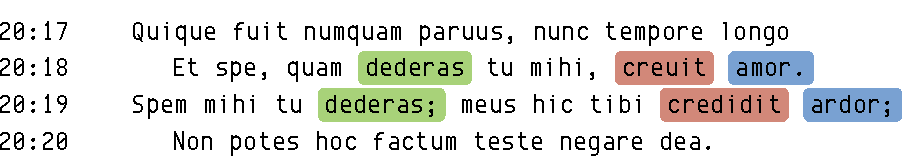
\includegraphics[width=0.48\textwidth]{heroides_pent.pdf}
\end{figure}

Overall, there is strong support for the view that ornamentation via vertical
rhyme \emph{was} consciously used, but with restraint. In hexameter, Lucretius
is the most significant user, but it is also a marked feature of the
\emph{Metamorphoses}. In elegiac couplets, vertical patterns were much more
common, with every author showing some propensity for them, in particular at
the line-initial position. 

\subsubsection{`Mosaic' Rhymes}
\label{sec:mosaic}

This feature-by-feature analysis is not enough to paint the full picture of
authorial style. Some of the most interesting rhymes occur when authors
combine \emph{multiple} rhymes in a dense passage of verse---what I will call
`mosaic rhymes'. Two examples of this type can be seen in Figs
\ref{fig:mosaic_phars} and \ref{fig:mosaic_aen}.

\begin{figure}[h]
    \caption{A dense mosaic quatrain from Lucan, \emph{Pharsalia} (score=8.50)}
    \label{fig:mosaic_phars}
    \centering
    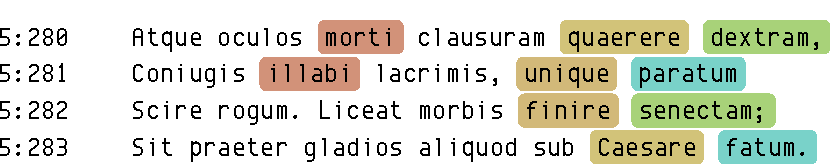
\includegraphics[width=0.48\textwidth]{phar_mosaic.pdf}
\end{figure}

\begin{figure}[h]
    \caption{Another mosaic, from Vergil's \emph{Aeneid} (score=7.65). Note also the echo \emph{quae me fuga} -- \emph{qui me mea}, which was beyond the scope of the automatic search.}
    \label{fig:mosaic_aen}
    \centering
    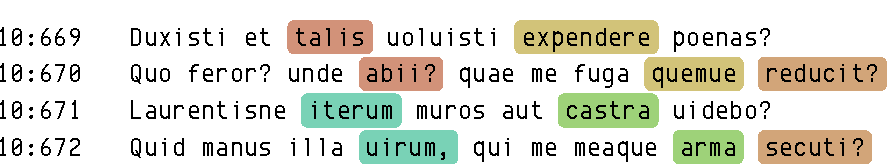
\includegraphics[width=0.48\textwidth]{aen_mosaic.pdf}
\end{figure}

 \citeA[139 ff.]{herescu_poesie_1960} gave some consideration to quatrain
patterns based on vertical assonance, but his analysis of dense passages of
rhyme (\emph{qua} rhyme) is more based on `horizontal' rhymes (p. 178). This
accords with his general belief that `rhyme occurs mainly in the final
position among modern poets, and in the interior position among the ancients'
\cite[175]{herescu_poesie_1960}.\footnote{
  `La difference [est] dans la place qu'on lui assigne dans le vers; elle est
  surtout \emph{finale} chez les Modernes, elle est surtout \emph{interieure}
  chez les Anciens' (original emphasis)
}
I have chosen to consider mainly vertical rhymes, with just the leonine
pattern for `interior' (i.e. horizontal) rhyme. Future work might look for
more powerful ways to connect these mosaic rhymes with authorial style.
\citeA[178]{herescu_poesie_1960}, for example, suggests that rhymes accumulate
`in passages with great sonic effect', but offers only \emph{Aeneid} 1.85--8
to serve as an example. Unfortunately, mosaic quatrains are moderately rare,
and so the statistical expectation for their counts is somewhat unreliable. To
quantify this `rarity', first recall that the quatrains are scored as a set,
based on both the number and the strength of rhyming positions. Taking a
quatrain score of 5.5 as a minimum threshold (see Fig. \ref{fig:phars_barely}
for an example that barely meets the threshold), there are about 22 mosaic
quatrains per thousand lines in the \emph{Aeneid}, 34 per thousand in the
\emph{Metamorphoses} and 28 in the \emph{Pharsalia}. Because there is no
precise definition of these mosaic rhymes, probabilities cannot be calculated
with the theoretical models, but simulation shows with more than 99\%
confidence that even the more modest number in the \emph{Aeneid} did not occur
by chance.\footnote{
  The greatest number in 101 simulated \emph{Aeneidae} was 20.12 per thousand,
  median 16.87.
}
In terms of broad trends (and this can be seen to some extent in Fig.
\ref{fig:rhymepca}), the elegiac works contain significantly higher rhyme
density than the hexameters, but the mean rhyme density is a different
statistic to the count of mosaics. For hexameters, the highest overall density
is in Lucan's \emph{Pharsalia}, followed at some distance by the
\emph{Thebaid} and the \emph{Metamorphoses}.

We may never have enough data to solidly connect these intricate
ornamentations to ideas of theme or poetic function,\footnote{
  As an experiment, I wondered whether rhyme density might be related to direct
  speech. I separated the \emph{Aeneid} into quoted speech vs narration and
  compared the average rhyme density, but found no compelling statistical connection.
}
but there is no doubt that they are worthy of attention in
criticism and philology. I remind the reader that the famous `golden line'\footnote{
  A five word line with a central verb, and two initial adjectives modifying
  two final substantives, i.e. abVAB. Consult
  \citeA[219--22]{winbolt_latin_1903} for several examples and some typical
  analysis. Amusingly, study of this form is entirely modern, emerging from the
  English philological tradition; on this, see \citeA{mayer_schoolboys_2020}.
}
is approximately ten times less common---there are just 34 in all ten thousand
or so lines of the \emph{Aeneid}---and yet they are a regular subject of
teaching and commentary. This study is limited, in this area, by the four line
`window' used in all of the tests. This was purely for pragmatic reasons---as
we widen our window for considering rhymes, it becomes difficult to tell the
noise from the signal. \citeauthor{deutsch_1978}, in her examination of
Lucretius, finds very long passages which are, in her analysis, part of a
single, extremely complex scheme. Some of these schemes include rhymes (and,
admittedly, very strong ones) which are ten or fifteen lines apart. There are
similar analyses in \citeA[149--76]{guggenheimer_rhyme_1972}, and again in
\citeA[176--8]{herescu_poesie_1960}. To properly test these ideas would
require more precise and quantifiable rules to include or exclude passages as
`extended rhyme schemes', but to automatically detect such extended matches
would be difficult with the approaches described here, due to the number of
false positives. This is not to say that it is out of the question, simply
that the scoring and analysis would need to be more sensitive and complex than
the basic approaches implemented so far.

\begin{figure}
    \caption{A mosaic which barely meets the threshold from the \emph{Pharsalia} (score=5.50)}
    \label{fig:phars_barely}
    \centering
    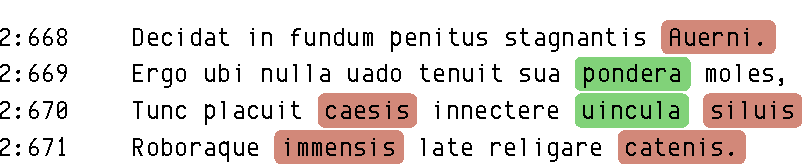
\includegraphics[width=0.48\textwidth]{phars_barely.pdf}
\end{figure}

\begin{table*}[h!]
\caption{
An analysis of the (almost universal) propensity ($\Pi$) for Leonine rhyme.
The test \texttt{slant\_leo} considers only rhymes that do \emph{not} share
common noun endings, like `-us', `-os', `-as' etc. Since the theoretical
probability for \texttt{slant\_leo} is impractical to calculate, the binomial
test is not performed and no $P$-value is calculated. This table includes
complete works only, where the statistics are less variable.
}
\label{tab:leo}
\par\medskip
\centering
% \resizebox{0.95\linewidth}{!}{
  \begin{tabular}{lclcccclcc@{\hspace{1\tabcolsep}}c@{\hspace{1\tabcolsep}}c}
  \toprule
          &&&&&&\multicolumn{3}{c}{Theoretical (Binomial)}&\multicolumn{3}{c}{Simulated}\\\cmidrule(lr{2pt}){7-9}\cmidrule(l{2pt}r){10-12}
         Work & Metre &       Test &    $\Pi$ & Signif. &    Obs. &  Exp. & Alt. &  $P$-val & L$_{95}$ &  M$_{50}$ &  H$_{95}$ \\
  \midrule
        Aeneid &     H &        leo & 1.2227 &   *** &  549 &       459 &     greater & <0.0001 &  422 &  449 &  491 \\
        Aeneid &     H &  slant leo & 1.1190 &   *** &  376 &         - &        - & - &  305 &  336 &  369 \\
    Apotheosis &     H &        leo & 1.6667 &   *** &   90 &        53 &     greater & <0.0001 &   39 &   54 &   68 \\
    Apotheosis &     H &  slant leo & 1.2368 &       &   47 &         - &        - & - &   27 &   38 &   50 \\
   Argonautica &     H &        leo & 1.6926 &   *** &  523 &       310 &     greater & <0.0001 &  279 &  309 &  344 \\
   Argonautica &     H &  slant leo & 1.3431 &   *** &  321 &         - &        - & - &  211 &  239 &  271 \\
           Ars &     H &        leo & 1.6765 &   *** &  114 &        67 &     greater & <0.0001 &   55 &   68 &   83 \\
           Ars &     P &        leo & 2.0135 &   *** &  149 &        71 &     greater & <0.0001 &   59 &   74 &   87 \\
           Ars &     H &  slant leo & 1.5849 &   *** &   84 &         - &        - & - &   42 &   53 &   65 \\
           Ars &     P &  slant leo & 1.3929 &   *** &   78 &         - &        - & - &   42 &   56 &   69 \\
           DRN &     H &        leo & 1.0467 &       &  336 &       325 &     greater & 0.2790 &  289 &  321 &  351 \\
           DRN &     H &  slant leo & 0.9440 &       &  219 &         - &        - & - &  204 &  232 &  266 \\
         Fasti &     H &        leo & 1.7357 &   *** &  243 &       138 &     greater & <0.0001 &  122 &  140 &  165 \\
         Fasti &     P &        leo & 2.1358 &   *** &  346 &       159 &     greater & <0.0001 &  144 &  162 &  182 \\
         Fasti &     H &  slant leo & 1.4762 &   *** &  155 &         - &        - & - &   90 &  105 &  128 \\
         Fasti &     P &  slant leo & 1.3443 &   *** &  164 &         - &        - & - &  106 &  122 &  149 \\
      Georgics &     H &        leo & 1.3426 &   *** &  145 &       110 &     greater & 0.0005 &   89 &  108 &  133 \\
      Georgics &     H &  slant leo & 1.3188 &    ** &   91 &         - &        - & - &   57 &   69 &   90 \\
  Hamartigenia &     H &        leo & 1.9778 &   *** &   89 &        45 &     greater & <0.0001 &   34 &   45 &   55 \\
  Hamartigenia &     H &  slant leo & 1.2500 &       &   40 &         - &        - & - &   22 &   32 &   43 \\
      Heroides &     H &        leo & 1.4444 &   *** &  156 &       107 &     greater & <0.0001 &   84 &  108 &  134 \\
      Heroides &     P &        leo & 1.8372 &   *** &  237 &       126 &     greater & <0.0001 &  106 &  129 &  157 \\
      Heroides &     H &  slant leo & 1.2262 &     * &  103 &         - &        - & - &   66 &   84 &  103 \\
      Heroides &     P &  slant leo & 1.1771 &       &  113 &         - &        - & - &   77 &   96 &  116 \\
     Hor. Sat. &     H &        leo & 1.2340 &     * &  116 &        99 &     greater & 0.0492 &   76 &   94 &  118 \\
     Hor. Sat. &     H &  slant leo & 1.1471 &       &   78 &         - &        - & - &   52 &   68 &   83 \\
     Juv. Sat. &     H &        leo & 1.5750 &   *** &  252 &       166 &     greater & <0.0001 &  135 &  160 &  188 \\
     Juv. Sat. &     H &  slant leo & 1.3471 &   *** &  163 &         - &        - & - &  101 &  121 &  139 \\
 Metamorphoses &     H &        leo & 1.3425 &   *** &  878 &       642 &     greater & <0.0001 &  607 &  654 &  695 \\
 Metamorphoses &     H &  slant leo & 1.1310 &   *** &  587 &         - &        - & - &  475 &  519 &  560 \\
     Pharsalia &     H &        leo & 1.2796 &   *** &  627 &       488 &     greater & <0.0001 &  446 &  490 &  532 \\
     Pharsalia &     H &  slant leo & 1.0355 &       &  379 &         - &        - & - &  328 &  366 &  393 \\
    Propertius &     H &        leo & 2.4355 &   *** &  302 &       126 &     greater & <0.0001 &  105 &  124 &  147 \\
    Propertius &     P &        leo & 2.4922 &   *** &  319 &       128 &     greater & <0.0001 &  105 &  128 &  150 \\
    Propertius &     H &  slant leo & 1.7349 &   *** &  144 &         - &        - & - &   65 &   83 &   99 \\
    Propertius &     P &  slant leo & 1.6129 &   *** &  150 &         - &        - & - &   75 &   93 &  110 \\
  Psychomachia &     H &        leo & 1.4444 &    ** &   65 &        46 &     greater & 0.0031 &   34 &   45 &   61 \\
  Psychomachia &     H &  slant leo & 0.9394 &       &   31 &         - &        - & - &   22 &   33 &   44 \\
        Punica &     H &        leo & 1.3130 &   *** &  818 &       628 &     greater & <0.0001 &  575 &  623 &  689 \\
        Punica &     H &  slant leo & 1.1253 &     * &  539 &         - &        - & - &  445 &  479 &  544 \\
       Thebaid &     H &        leo & 1.4486 &   *** &  775 &       536 &     greater & <0.0001 &  494 &  535 &  583 \\
       Thebaid &     H &  slant leo & 1.1785 &   *** &  482 &         - &        - & - &  367 &  409 &  443 \\
      Tibullus &     H &        leo & 1.1463 &       &   47 &        39 &     greater & 0.1090 &   28 &   41 &   53 \\
      Tibullus &     P &        leo & 2.0000 &   *** &   80 &        40 &     greater & <0.0001 &   29 &   40 &   53 \\
      Tibullus &     H &  slant leo & 0.9697 &       &   32 &         - &        - & - &   21 &   33 &   44 \\
      Tibullus &     P &  slant leo & 1.2143 &       &   34 &         - &        - & - &   21 &   28 &   41 \\
       Tristia &     H &        leo & 1.3936 &   *** &  131 &        91 &     greater & <0.0001 &   76 &   94 &  115 \\
       Tristia &     P &        leo & 2.0168 &   *** &  240 &       114 &     greater & <0.0001 &  100 &  119 &  142 \\
       Tristia &     H &  slant leo & 1.0735 &       &   73 &         - &        - & - &   53 &   68 &   87 \\
       Tristia &     P &  slant leo & 1.3368 &   *** &  127 &         - &        - & - &   78 &   95 &  114 \\
  \bottomrule
  \end{tabular}
% }
\end{table*}

\subsubsection{Leonine Rhymes (Table \ref{tab:leo})}
\label{sec:leo}

Almost every work shows a statistical propensity for the `leonine' rhyme. In
this study I accept as leonine any rhyme that occurs between a word ending at
a third-foot caesura (whether weak or strong) and the final word of the line.
The first and most important thing to discuss is the idea that leonine rhymes
occur `naturally' due to agreement with nouns in the mid or final positions.
Proponents of this view might present lines such as this one:
\begin{adjustwidth}{0.5cm}{0.5cm}
  et me saeuus \emph{equis} Oriens afflauit \emph{anhelis}

  \noindent and savage Morning breathes on me \emph{with panting steeds}
  \begin{flushright}
    \emph{Aen.} 5.739
  \end{flushright}
\end{adjustwidth}
Therefore, it is claimed, the leonine rhymes we see are not consciously
sought; as argued by \citeA[34]{wilkinson_golden_1963} they simply `strike us
more forcefully' due to the widespread use of this rhyme in regular forms in
medieval verse. 

Based on this proposition, we would expect natural `inflation' in the number
of leonine rhymes, since they are (the argument goes) a natural consequence of
adjectives occurring near the nouns they modify. I do not believe this is
enough to explain away the clear preference of almost every author, or indeed
the very marked increase in propensity seen in elegy vs epic (even in the
hexameter). I also note that we do \emph{not} see a propensity for leonine
rhyme in Lucretius' \emph{De Rerum Natura} ($\Pi=1.05$). If the leonine style
of rhyme were indeed inevitable then it is unlikely that Lucretius should have
produced almost six thousand lines of hexameter without displaying this
feature---and so even if such inflation exists then it is slight.

\citeA[49]{platnauer_latin_1951} claims that this \textsc{adj}-\textsc{nom} agreement accounts
for around 90\% of the rhymes.\footnote{
  Platnauer only considered the pentameter, but as can be seen in Table
  \ref{tab:leo}, Ovid and Propertius both use this feature in their hexameters
  as well, where the metre is more flexible. The central caesura in the
  pentameter is obligatory, and an \textsc{adj}-\textsc{nom} agreement with a
  rhyme is often used to `balance' a line, but this should hardly be seen as
  accidental.
}
Based on a random sample of pentameters from the \emph{Fasti} which I analysed by
hand, and using my (probably more permissive) threshold for `rhyme', I would
suggest that his figure is a little high,\footnote{
  See also the figures from several other sources collected in \citeA[33 in
  note]{wilkinson_golden_1963} which vary considerably, and measure a variety
  of slightly different things.
}

but not sufficiently so as to invalidate his point. The only way to
conclusively settle the matter would be to perform part-of-speech (POS)
analysis of the entire corpus being analysed, and to determine how often this
\textsc{adj}-\textsc{nom} agreement takes place. However while automatic POS
analysis for Latin has taken some great leaps recently,\footnote{
  Of particular interest are the joint learning framework PIE
  \cite{manjavacas-etal-2019-improving} and the model and Python API that is
  pre-trained for Latin by \citeA{thibault_clerice_2020_3883590}.
}
even perfect POS tagging would not completely solve the problem---it may
be that a pair of words `match' grammatically (i.e. in number, gender, and
case) and yet the adjective actually modifies a different substantive
altogether. So, with some regret, this investigation is deferred to future
work.

What \emph{was} possible was a very coarse workaround. The test
\texttt{slant\_leo} simply scans for leonine rhymes \emph{except} those in
which both words end with a common nominal suffix (-os, -is, -as, etc.). This
test would not match \emph{equis--anhelis} in the line quoted above. The
hypothesis is then that authors who show a clear preference for both
\texttt{leo} and \texttt{slant\_leo} really are exhibiting a significant
tendency. Note that this test does not exclude \emph{all} of the `90\%' of
rhymes claimed by Platnauer, since it does not reject words where the
grammatical correspondence is revealed by a single letter (in particular,
ablatives and genitives ending -a, -i, -o), but rejecting those rhymes
entailed too many false positives.

Personally, I take at face value the statistics in Table
\ref{tab:leo}---showing that leonine rhyme occurs more frequently than chance
would suggest throughout classical Latin verse. In any case, despite any
inevitable inflation, there is still great value in the comparative study of
the style of the various poets, and also in considering the diachronic
development of the pattern. Leonine rhyme is strongest in the elegists and, in
those, more so in the pentameter (although note the difference between say
Propertius, strongly leonine in both metres, and Tibullus who shows a more
traditional hexameter). In pure hexameter, the most enthusiastic users of the
leonine pattern are Valerius Flaccus in the \emph{Argonautica} and the
\emph{Satires} of Juvenal. One might begin to wonder if this is simply a trend
that grew more common over time---and indeed this may well be the case. The
fly in that particular ointment is the much earlier Catullus 64; with a $\Pi$
of $1.54$, it is more leonine than any classical work except the two just
mentioned. It is, however, only 406 lines long, and so we might simply be
looking at random variation. For the sake of interest, I included a few fourth
century (\textsc{ce}) works by Prudentius, and they are, indeed, more leonine
than all of the classical hexameter. The \emph{Apotheosis} displays a $\Pi$ of
$1.73$ and the \emph{Hamartigenia} $1.93$ (both poems contain about 1000 lines
of hexameter, roughly the same as a single book of classical epic). At the end
of the day, the evidence comes from a relatively small number of texts. All
the same, it may be worth investigating additional Late Antique verse to see
if this trend might continue. It does seem only natural that the regular
leonine pattern `invented' by Gottschalk in the ninth century should be more
of an evolution than a sudden innovation---another area for future work.

\subsection{Multivariate Analysis and Visualisation}

For the multi-variate analysis, each work was represented by the vector
containing its $\Pi$ scores for each test, along with the global scores
\texttt{rhyme amount} and one for \texttt{rhyme score}, as discussed above in
Section \ref{sec:whole_rhyminess}. There is a small procedural wrinkle, here,
because works that are in elegiac couplets have two scores for each test (one
for the rhyme test commencing at a hexameter line, e.g. \texttt{H-aa -1}, and
one for the same test commencing at a pentameter line, \texttt{P-aa -1})
whereas hexameter works are written in a single metre. Since the vectors to be
considered must all contain the same number of components, the hexameter
vectors were `doubled in length' by simply repeating the scores for the
hexameter tests. This might create an artificial difference between works
written in hexameter and works in elegiac couplets---and so the fact that the
elegiac works cluster together is perhaps not entirely an artefact of
authorial style. From a careful inspection of the univariate results, however
(Tables \ref{tab:allbutleo} and \ref{tab:leo}) it is clear that elegiac works
were genuinely different; in particular in the number of leonine rhymes and
also the propensity towards rhymes (or repeats) in the initial position
(\texttt{aa 0}, \texttt{axa 0} etc.). The final vector for each work has 30
components---28 $\Pi$ scores for 14 different rhyme tests (see Table
\ref{tab:df_apot}) and two global scores for general rhyminess. As a reminder,
the $\Pi$ scores are left unchanged, but the global rhyme scores are
standardized to a zero mean and unit variance using the scikit-learn
\texttt{StandardScaler} \cite{scikit-learn}.

\begin{figure*}[ht]
\caption{
  UMAP Cluster of works, scaled by size and coloured by work. Nearby works are
  stylistically similar in the way they use rhyme. Long works are shown as
  whole units (larger) and also in their individual books, to highlight the
  stylistic variation that can occur.
}
\label{fig:rhymecloud}
\centering
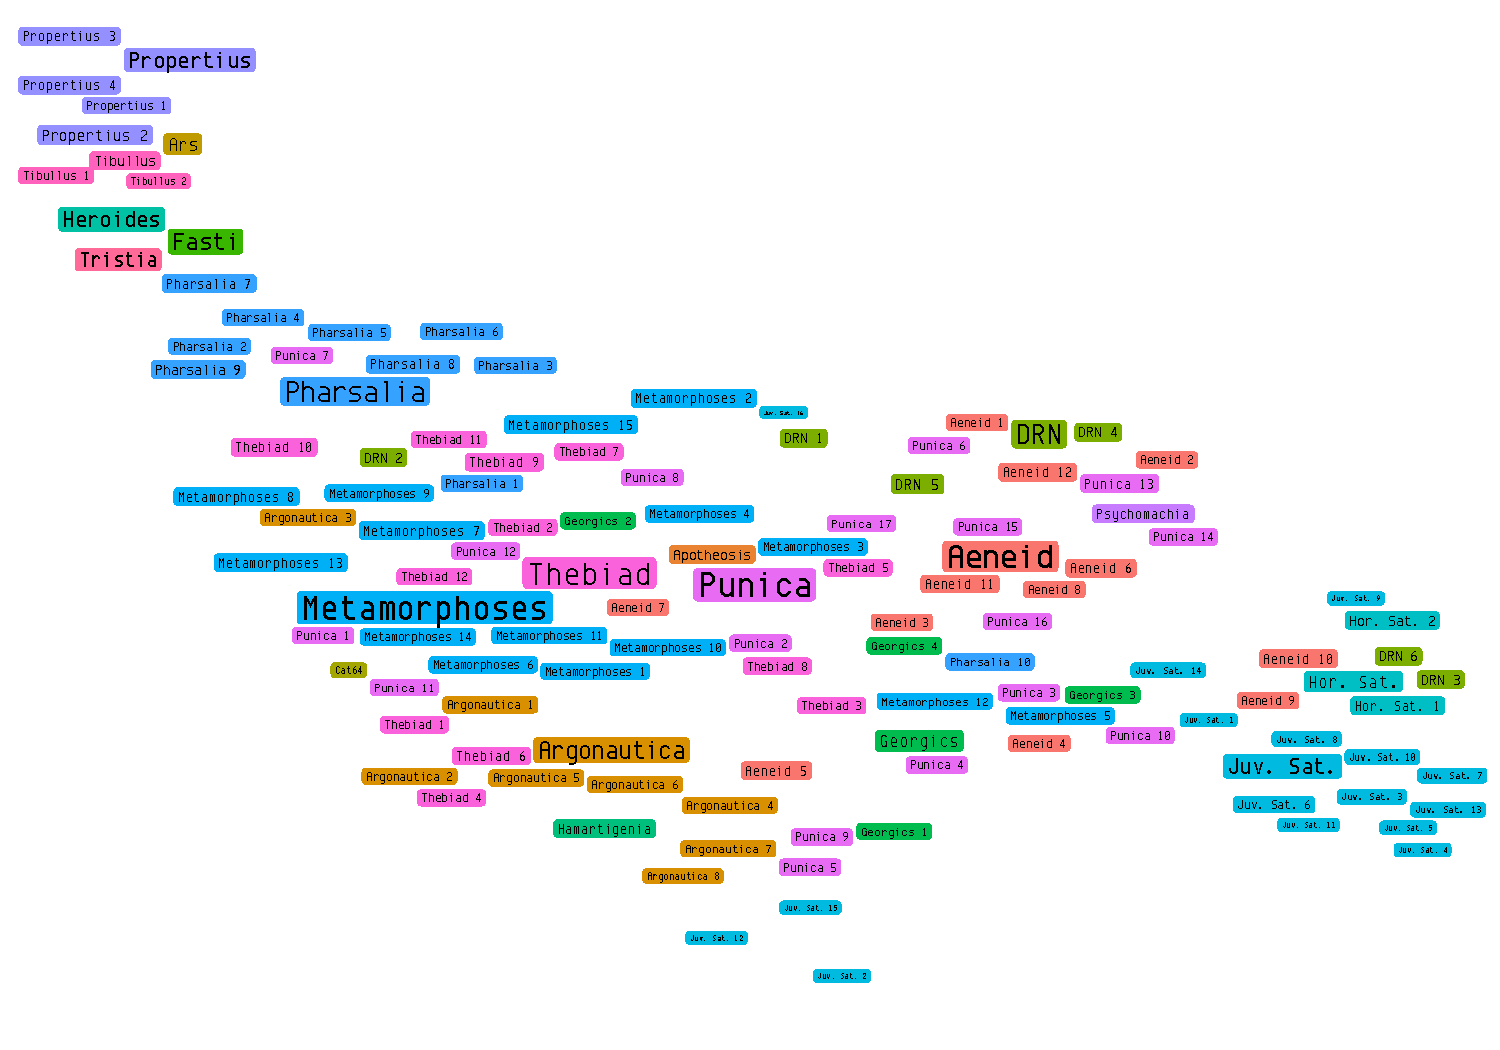
\includegraphics[width=0.8\textwidth]{rhyme_umap.pdf}
\end{figure*}

\subsubsection{UMAP (Manifold Projection) Clustering (Fig. \ref{fig:rhymecloud})} 

For the first analysis, the works were analysed with unsupervised clustering
using UMAP \cite{mcinnes_umap_2018}. UMAP is a manifold projection tool, which
(roughly) means that when we project down to a two-dimensional figure, it
attempts to preserve small-scale local distances between points in the high
dimensional space as best it can. Conceptually it is somewhat similar to t-SNE
(in that it considers local distances instead of trying to determine centroids
like \emph{k-means}) but UMAP is easier to tune and works well for a quick
visualisation. In Fig. \ref{fig:rhymecloud}, each work is plotted separately,
and scaled by size. Nearby works are `close' to each other, but relative
distances for distant works should probably be treated with caution, i.e. it
is not necessarily true that Juvenal's \emph{Satires} are \emph{more} similar
to the \emph{Punica} than Lucan's \emph{Pharsalia}, but it is fair to say that
the \emph{Metamorphoses} and the \emph{Thebaid} are close.

Based on a number of experiments (which are omitted for brevity) and also on
the PCA analysis in the following section, the most important general
differentiator (moving from right to left) is the overall rhyme density---the
\emph{Satires} of Juvenal and Horace being the least dense, Lucan's
\emph{Pharsalia} the densest of the epics and then the elegiac works the
densest of all. In this figure, however, the most useful things to think about
are the local relationships between the works. There are a number of
interesting observations.

There is a clearly visible division between the three broad genres: elegy,
satire and epic. This is particularly interesting in terms of Ovid, who wrote
in several different modes: `epic' (if one can be forgiven for so broadly
characterising the \emph{Metamorphoses}), love elegy (the \emph{Ars} and the
\emph{Heroides} although again an over-simplification), and didactic
elegy (the \emph{Fasti}) just to take a few examples. Despite the different
tone of Ovid's elegiac works, they cluster tightly together, whereas the
\emph{Metamorphoses} sits somewhere in the middle of the spread of
`traditional' epic. Unfortunately, Ovid is the only author who was this
flexible---the rest wrote elegy or epic, but not both.\footnote{
  This is unfair to Horace, of course, who was extremely flexible in moving
  between the Greek metres and the dactylic hexameter of his \emph{Satires}, as
  was Catullus with hendecasyllables versus his hexameter epyllion Cat. 64, but
  the point stands with respect to the two metres that were analysed in this
  study.
}
Never the less, it is reasonable to conclude that there is some sort of link
between the way in which rhyme was handled and the mode of the verse being
written. This further underlines the fact that there was a conscious awareness
of rhyme.

Within the broad clusters, authorial style can vary a great deal. In some
cases like the \emph{Argonautica} and \emph{Pharsalia}, individual books
cluster fairly closely to the vectors representing the entire work (shown
larger in the figure). In others, and probably most obviously with the
\emph{Punica} it is clear that there is very significant variation from book
to book. The feature space used for this project seems to \emph{broadly}
separate works, but a significant amount of text would be required before
attempting tasks like authorship attribution or forgery detection. This is not
to say that the approach evaluated here would be useless for such tasks, but
more to suggest that it would not be suitable in isolation, but better as a
part of broader, multi-mode expression of style.

The final thing I will note is that there is no clear temporal signal in Fig.
\ref{fig:rhymecloud}. The elegiac works, in any case, were written within a
fairly short historical period, but the hexameters of the \emph{Aeneid} and
the \emph{Punica} cluster nearby, despite being separated by roughly a
century. What is more, Vergil's earlier \emph{Georgics} appear in that zone,
as well as the \emph{Psychomachia} of Prudentius, one of the three Late
Antique works from the fourth century \textsc{ce}. The \emph{Argonautica} and the
\emph{Thebaid} are reasonably close (two of the three works of Flavian epic)
but so are the \emph{Satires} of Horace and Juvenal, once again written more
than a century apart. This should probably be no surprise, of course, since
Horace was almost certainly one of Juvenal's influences. And so, these
features do not seem particularly well-matched to questions of dating or
priority. Having said that, and as mentioned before, it may be possible that
\emph{individual} features (such as the use of leonine rhyme) became more or
less common over time---but that should be analysed via the univariate
statistics. This is not to say that the apparent division in the epic works is
useless---it appears that a case could be made for a `traditional' model based
on Vergil (to whom Silius owed a great stylistic debt) and a more progressive
model encompassing Ovid, Statius, Lucan and Valerius Flaccus. The following
analysis via PCA has more to say on this subject but essentially the idea,
although interesting, requires more investigation.

\begin{figure*}[ht]
    \caption{
    Principal Component Analysis (PCA) plot of the same data from Fig.
    \ref{fig:rhymecloud}. \texttt{PC1} and \texttt{PC2} account for 72\% of
    the explained variance. In order to preserve legibility it was necessary
    to avoid over-plotting, so some works may be closer to the origin than
    they appear, but the relative direction of their displacement is
    preserved. Inset: the relative direction of the most important features.
    }
    \label{fig:rhymepca}
    \centering
    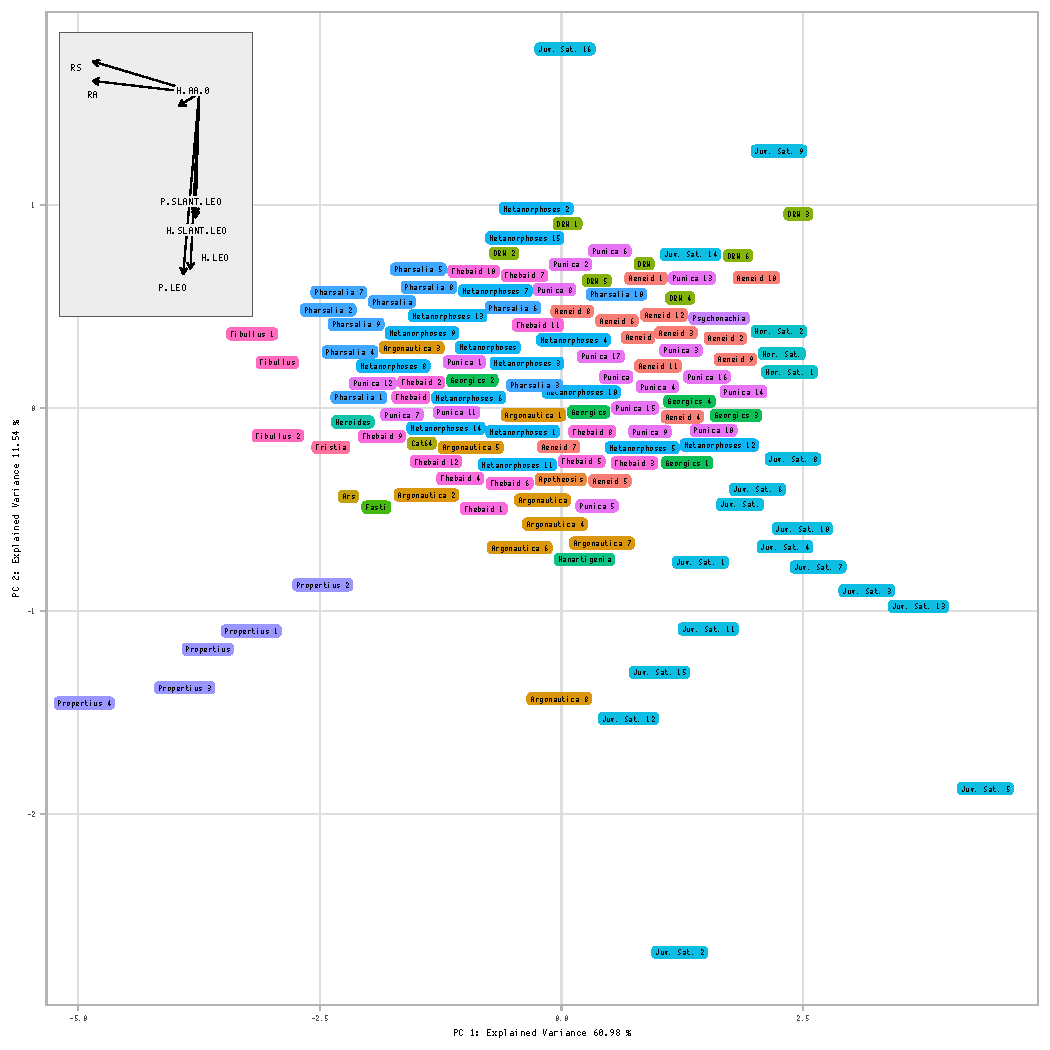
\includegraphics[width=0.8\textwidth]{rhyme_pca_arrows.pdf}
\end{figure*}

\subsubsection{A Principal Component Analysis (PCA) (Fig. \ref{fig:rhymepca})}

A standard visualisation technique to explore multi-variate relationships is
Principal Component Analysis (PCA). While the previous section tried to give
insight into the way the various works relate to each other, PCA can often
provide some understanding as to how the data is separated by the individual
features. This is not the place for a full explanation of the technique, but
some broad intuition may assist the reader. The `principal components' (hence
PCs) are \emph{composite} features; each PC comprises some element of several
of the `true' features. Because of the nature of the mathematical
construction, the full set of PCs separate the data well in high dimensional
space, but the real value of them in terms of visualisation is that the PCs
are \emph{ordered} in terms of how well they perform this separation. So, by
plotting the data against the first two PCs, we often obtain a useful
projection of high dimensional data in a two-dimensional plot. In this case
the PCA is very informative---the first two PCs account for 72\% of the
observed variation (so they are very descriptive) and they are each dominated
by essentially a single feature (so they are easy to understand). In Fig.
\ref{fig:rhymepca}, \texttt{PC1} is dominated by the two features describing
rhyme density (scores $<0$ have more rhyme overall) and \texttt{PC2} is
dominated by the propensity for leonine rhyme (scores $<0$ are more leonine).
So, for the sake of orientation, Propertius 3 is both unusually rhymey and
leonine, Juv. \emph{Sat.} 9 is unusually free of both, Juv. \emph{Sat.} 5 is
very leonine but with low rhyme density, etc. Hopefully, for a reader armed
with that information, the figure may now speak for itself, but here are a few
observations of my own.

In the UMAP visualisation (Fig. \ref{fig:rhymecloud}), the elegiac works
clustered tightly overall, showing a fundamental difference in the way rhyme
was handled between elegy and epic. In the PCA figure, we can begin to tease
apart the styles of those authors. Tibullus and Propertius are both towards
the high end for rhyme density, but are quite different in the degree to which
they use leonine rhymes. This can also be seen in the descriptive statistics
in Table \ref{tab:leo}---in particular, Tibullus is much more sparing of this
ornamentation in his hexameters. Ovid, we now see, appears to use the leonine
style more in the \emph{Ars} and \emph{Fasti} than the \emph{Heroides} or the
\emph{Tristia}. In a similar vein, the \emph{Satires} of Horace and Juvenal,
which exhibit a high degree of self-similarity in the UMAP clusters, can be
differentiated once again by their handling of leonicity---but in contrast to
elegy they both have low rhyme density. As an aside, it seems
counter-intuitive for Juvenal to have such a strong $\Pi$ for leonine rhymes
but a low overall density; the explanation appears to be that this is the only
rhyming ornament that Juvenal employs with any regularity---the `mosaic' rhymes
employed to a varying degree by the epicists are rare in Juvenal.\footnote{
  Using the same threshold as in Section \ref{sec:mosaic} there are 16.6 per
  thousand, compare the \emph{Aeneid} 21.8, \emph{Metamorphoses} 34.1, and
  \emph{Pharsalia} 28.4. This number is close to the simulated median,
  suggesting no detectable propensity (nor a detectable aversion).
}

Works near the centre of the plot are not strongly characterised. The PCA
gives more weight to features which \emph{separate} works, and in this case
that task is dominated by the two features we have just discussed (leonicity
and rhyme density). The individual tests for various kind of vertical rhyme,
as seen in Table \ref{tab:allbutleo} are drowned out in this figure, even when
the $\Pi$ scores are clearly significant. Neither this figure nor the the UMAP
plot is wholly satisfactory, which is why it is useful to consider the data
through a number of different visualisations. And, of course, the
visualisations that can be printed on paper are only simplified projections of
data models that exist in high-dimensional space, so it is inevitable that
some information be lost.

\section{Conclusions}
\label{sec:conclusion}

The primary goal of this paper has been to break a small area of new ground in
the computational study of Latin verse. By providing an initial set of tools
and algorithms for the detection and statistical analysis of rhyme it is hoped
that future work will have an easier path to follow. The tools, data and
replication information are available from the associated code repository
\cite{nagy_rhyme_2021}. This study shows that, for classical Latin verse, the
baseline levels for rhyme are heavily affected by positional constraints. To
this end it introduces a Propensity Index, $\Pi$, which facilitates
comparative analysis in a way that percentages cannot. Incremental advances to
the technical approaches would be valuable, and the way is now (more) open for
studies that aim to verify, dispute, deepen or extend the rich tradition that
exists in Classical scholarship. The analysis presented has been mostly aimed
at establishing some fundamental claims, using a corpus whose breadth, finally,
can be claimed to be generally representative.

The key result of the analysis, which will seem tiresomely obvious to some, is
that rhyme \emph{is} part of the authorial fingerprint for classical Latin
verse. Far from the idea that authors avoided rhyme, or even the idea that
`rhyme simply happened by chance' it is clear that rhyme was used differently
by different authors and differently in different genres. This finding should
validate and encourage further study into the particulars; why is the Tibullan
hexameter less leonine than the Propertian? Why does Propertius `unify' his
couplets with vertical rhyme where Ovid is more inclined to link them? Why is
line-initial rhyme more favoured in elegy than epic? What literary effects are
supported by these technical devices? 

The study of concentrated `mosaic' rhymes (Section \ref{sec:mosaic}) is a
nascent attempt to apply formal quantitative analysis to the idea of `extended
schemes' typified by \citeA{deutsch_1978} and \citeA{guggenheimer_rhyme_1972}.
 The initial work here is limited by the four-line window, which seeks to find
individual mosaics that `stand out' from larger passages of text. Different
approaches will be needed to consider the long, extended schemes, and it is
not yet clear how far this can be taken. \citeA[148]{deutsch_1978}, at one
point, concludes that `the whole of Lucretius is one great scheme of rhyme'
and that it is `difficult to appreciate completely the close interweaving of
similar words and sounds, unless the entire passage can be read aloud' (p.
147). This is probably true for computational analysis as well---there is only
so much a computer can do, and still an irreplaceable role for the ear of a
human critic. Never the less there is an obvious benefit to using automated
tools to quickly scan long works for candidate passages. With respect to
Deutsch's `close interweaving of similar words and sounds', and based on a
fairly shallow exploration of the literature, an interdisciplinary approach
that incorporates related work on rap lyrics appears to show potential; their
problems are very much like the ones faced here.

In terms of computational stylometry, the authorial signal that can be
identified with the methods described here is not very strong. No attempt was
made to classify works, but based on the unsupervised clustering methods,
comparatively large samples would be needed. Even when taking entire books as
observations (a book of hexameter epic is typically 4--5000 words) there is a
great deal of stylistic variation. In some cases, good results may be possible
for one-vs-one determinations, but in general it appears more sensible to
consider adding rhyme as one component to a multi-faceted representation of
style. Perhaps, in the final assessment, this paper poses more questions than
it is able to conclusively answer. None the less, it is hoped that these
findings and new tools might justify and support further research into
an area of Latin poetics that has hitherto been consigned to the fringes of
the field.


%%%%%%%%%%%% Supplementary Methods %%%%%%%%%%%%
%\footnotesize
%\section*{Methods}

%%%%%%%%%%%%% Acknowledgements %%%%%%%%%%%%%
%\footnotesize
%\section*{Acknowledgements}

%%%%%%%%%%%%%%   Bibliography   %%%%%%%%%%%%%%
\normalsize
\bibliography{digilat}

%%%%%%%%%%%%  Supplementary Figures  %%%%%%%%%%%%
%\clearpage

%%%%%%%%%%%%%%%%   End   %%%%%%%%%%%%%%%%
%\end{multicols}  % Method B for two-column formatting (doesn't play well with line numbers), comment out if using method A
\end{document}
